\documentclass{article}
\usepackage{graphicx} % Required for inserting images
\usepackage{amsfonts} %used for the mathbb command
\usepackage{amsmath}

\usepackage[a4paper, margin=1in]{geometry} % Adjust margins here

\title{Characterizing Filamentary Structures in Turbulent Magnetohydrodynamic Simulations: \\
{Mid Semester Report}}
\author{Sasi Mitra Behara}
\date{\today}

\begin{document}

\maketitle

\begin{abstract}
The interstellar medium (ISM) of galaxies consists of filamentary structures where stars can form. To completely understand the role of such structures in star formation and gas dynamics, it is essential to characterize their sizes and shapes. With this motivation, we will use turbulent magnetohydrodynamic simulations, representing a typical part of a Milky Way-type galaxy, and characterize filaments using Minkowski functionals.
\end{abstract}


\section{Introduction}

The interstellar medium (ISM) of galaxies is a complex environment composed of thermal gas, dust, turbulence, magnetic fields and cosmic rays, characterized by filamentary structures in several of these components that play a crucial role in the process of star formation. Understanding the properties of these filaments, such as their sizes, shapes, and dynamics, is essential for unraveling the mechanisms underlying star formation and gas dynamics in galaxies. Recent advancements in turbulent magnetohydrodynamic (MHD) simulations have provided valuable insights about ISM.

To effectively characterize the filaments present in the simulation data, we employ Minkowski functionals, which serve as a generalized method for quantifying geometric properties. For 3d structures, the properties are volume, surface area, mean curvature, and the Euler characteristic. These functionals can be used to derive additional metrics, including planarity and filamentarity, which are critical for understanding the structure and morphology of the filaments within the ISM.

This report summarizes the development of a generalized code designed to compute the planarity and filamentarity of objects embedded in a three-dimensional space. This code can then be used to analyze the data produced in both the simulations and ISM observations.

\subsection{Project Outline}
The Simulation data comes from the following paper \cite{DataPaper}, where, using numerical simulations the authors explore the properties of turbulence for subsonic and supersonic turbulent flows. 

We can identify iso-density surfaces, where the density, or any other simulation parameter has the same value throughout the surface. Figure \ref{fig:b_field_isosurfaces} shows an illustration of what such iso-surfaces may look like \cite{AmitSetaThesis}. By choosing an appropriate value, we can isolate the filaments and then characterize them using Minkowski Functionals. 


\begin{figure}[h!]
    \centering
    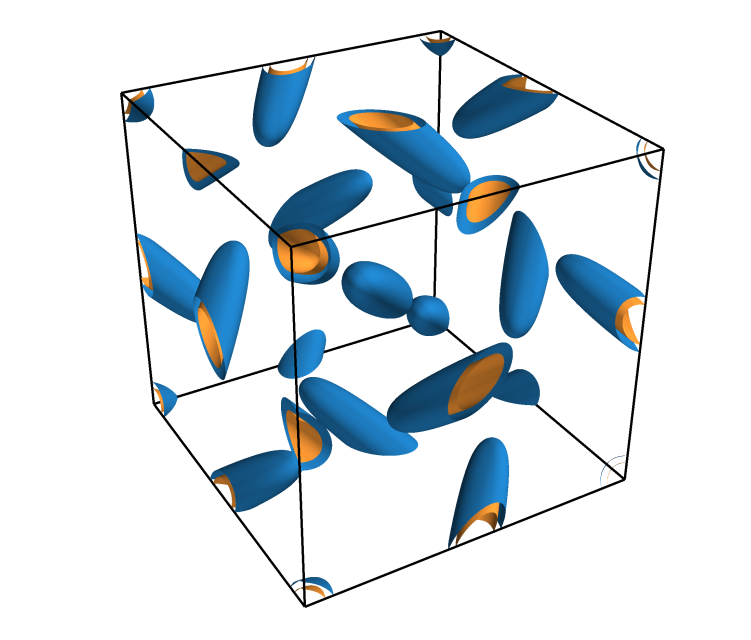
\includegraphics[width=0.5\textwidth]{Images/b_field_isosurfaces.png}
    \caption{Iso-surfaces of magnetic fields, where $b/b_{rms} = 2$ is marked in Blue, and $b/b_{rms} = 3$ is marked in yellow, from simulation data. Similar surfaces can be constructed for the data we are interested in, and characterize their properties. Image Source Figure 2.35 of \cite{AmitSetaThesis}}
    \label{fig:b_field_isosurfaces}
\end{figure}



The initial part of the project focused on developing code to calculate the shapefinders for a given data cube and testing the code for its validity.

\section{Minkowski Functionals}
Minkowski functionals are a set of mathematical tools used to analyze the shape and structure of data, in a variety of fields, including cosmology and astrophysics \cite{1999PaperMinkowskiFunctionalsInCosmology}. These functionals measure the geometric properties of sets and can describe the morphology of complex structures. In cosmology, Minkowski functionals are particularly valuable for studying the large-scale structures of the universe and the connectivity of cosmic structures. Here, we use similar techniques to identify and characterize filamentary structures.


\subsection{Hadwiger's Theorem}
In Integral Geometry, Hadwiger's Theorem characterizes the valuations on convex bodies in $\mathbb{R}^n$. Hadwiger's Theorem is a seminal result in integral geometry that provides a comprehensive characterization of valuations on convex bodies in $\mathbb{R}^n$. The theorem states that any continuous, translation-invariant valuation defined on the space of convex bodies embedded in $\mathbb{R}^n$ can be represented as a linear combination of a set of $n+1$ valuations, known as Minkowski Functionals \cite{adler_taylor_2007}.

Minkowski Functionals are a series of geometric measures that capture essential properties of convex shapes. In 3d Space ($\mathbb{R}^3$), The geometric interpretations of all Minkowski functionals in three dimensions are summarized in Table \ref{table:table_of_formulae} 

\begin{table}[]
\centering
\begin{tabular}{|l|l|l|l|}
\hline
\textbf{$\mu$} & \textbf{$V_\mu$} & \textbf{Geometric Interpretation} & \textbf{Crofton Formulae for Sphere} \\ \hline
0              & V                & Volume                            & $4/3 \pi r^3$                \\ \hline
1              & A/6              & Surface Area                      & $2/3 \pi r^2$                  \\ \hline
2              & H/$3\pi$         & Mean Curvature                    & $4/3r$                        \\ \hline
3              & $\chi$           & Euler Characteristic              & 1                                    \\ \hline
\end{tabular}
\caption{Table of the Various Minkowski Functionals, and the corresponding Crofton's Formulae for a sphere \cite{AmitSetaThesis}}.
\label{table:table_of_formulae}
\end{table}


\subsection{Shapefinders}
An important task of morphological statistics is to quantify non-random features such as filaments and pancakes. Given the four Minkowski functionals, we aim to reduce the morphological information they provide, to two measures: planarity, and filamentarity. \cite{Schmalzing1999}

Starting with the three independent ratios of the Minkowski funtionals, we get qualities that have a dimension of length. Requiring that these ratios give us the radius R if applied to a Sphere, we get three length scales
\begin{equation}
    l_0 = \frac {V_0}{2V_1}, \: \:\:
    l_1 = \frac {2 V_1}{\pi V_2}, \:\:\:
    l_2 = \frac {3 V_2}{4 V_3}
\end{equation}

By arranging the three length (L), width (W) and thickness (T) such that $L \ge W \ge T$, we can now define dimensionless shapefinders by 
\begin{equation}
    p = \frac {W - T}{W + T}, \: \: \:
    f = \frac {L - W}{L + W}
\end{equation}

These shapefinders give us information about how pancake-like and how filament-like the objects embedded in the given volume are. They take values between 0 and 1, such that a Flat Disc would have $p = 1, f = 0$. A cylinder would have $p = 0, f = 1$. A sphere would have $p = 0, f = 0$. 

\section{QuantimPy Library}
QuantImPy is a python library designed for scientific image processing. It performs morphological operations on numpy arrays and computes Minkowski functionals and functions. Inspired by the QuantIm C/C++ library, QuantImPy offers a user-friendly interface for handling complex image analysis tasks. The library is particularly useful for researchers and developers working with 2d and 3d image data, providing robust tools for quantitative analysis. \cite{boelens2021quantimpy}

The library takes input of a 3d boolean array, which represents the 3d space, and the locations of the structure of interest embedded in the space is marked with a True, while free space (not belonging to the structure of interest) is marked as False. The library then solves integrals \ref{eq:M_0}, \ref{eq:M_1}, \ref{eq:M_2}, \ref{eq:M_3} to obtain the Minkowski Functionals \cite{quantimpy_minkowski}

\begin{equation}
    M_0(X) = \int_X dv, \\
    \label{eq:M_0}
\end{equation}
\begin{equation}
    M_1(X) = \frac{1}{8} \int_{\delta X} ds,
    \label{eq:M_1}
\end{equation}
\begin{equation}
    M_2(X) = \frac{1}{2\pi^2} \int_{\delta X} \frac{1}{2} \left[ \frac{1}{R_1} + \frac{1}{R_2} \right] ds \:\:\: \text{and}
    \label{eq:M_2}
\end{equation}
\begin{equation}
    M_3(X) = \frac{3}{(4\pi)^2} \int_{\delta X} \left[ \frac{1}{R_1 R_2} \right] ds
    \label{eq:M_3}
\end{equation}

\subsection{Normalization and Developing a Wrapper Function}

Solving the equations provided in the documentation for the case of a Sphere of Radius $R$, we see the equations reduce to the following:
\begin{equation}
    M_0 = \frac 4 3 \pi r^3
\end{equation}
\begin{equation}
    M_1 = \frac 1 8 4 \pi r^2
\end{equation}
\begin{equation}
    M_2 = \frac {2 r}{\pi} 
\end{equation}
\begin{equation}
    M_3 = \frac {3}{4 \pi}
\end{equation}

Comparing these with the Crofton Formulae \cite{AmitSetaThesis} for the same quantities,
$$V_0 = \frac 4 3 \pi r^3, \:\: V_1 = \frac 2 3 \pi r^2, \:\: V_2 = \frac 4 3 r, \:\: V_3 = 1$$

We know the two values are off by a a normalizing factor, since they both represent the same quantities. Dividing them, we obtain the quantities as
\begin{equation}
    N_0 = 1, \: \: N_1 = \frac 4 3 ,\: \: N_2 = \frac {2 \pi}{3} ,\: \: N_3 = \frac{3}{4 \pi} 
\end{equation} 

Such that, $V_\mu = N_\mu * M_\mu$, where $V_\mu$ is the corresponding Crofton Formula, which we need for calculating the shapefinders, and $M_\mu$ is the corresponding Minkowski Fucntional calculated by the library.


Wrapper functions in python were created to calculate these Functionals and convert them into the convenient forms, and additional python functions to calculate the Filamentarity and Planarity were also developed. These functions were tested for the case of a Sphere to ensure that the outputs match what is expected, and the outputs have been tabulated in Table \ref{tab:wrapper_function_outputs}. The differences between the Analytical and Computed Values are attributed to the numerical errors, and are sufficiently small.

\begin{table}[]
	\centering
	\begin{tabular}{|l|l|l|}
		\hline
		\textbf{Function} & \textbf{Computed Value} & \textbf{Analytical Value} \\ \hline
		$V_0$             & 1767063.00              & 1767145.87                \\ \hline
		$V_1$             & 11777.28                & 11780.97                  \\ \hline
		$V_2$             & 100.28                  & 100.00                    \\ \hline
		$V_3$             & 1.00                    & 1.00                      \\ \hline
		T, W, L           & 74.77, 75.02, 75.21     & 75.00, 75.00, 75.00       \\ \hline
		Planarity         & 0.00                    & 0.00                      \\ \hline
		Filamentarity     & 0.00                    & 0.00                      \\ \hline
	\end{tabular}
	\label{tab:wrapper_function_outputs}
	\caption{The Minkowski Functionals, the length scales, and the Planarity and Filamentarity, calculated by the code and the analytical formulae, for a sphere of radius 75m, embedded in a grid of $300^3 m^3$.}
\end{table}


\section{Radius Variance of Minkowski Functionals}

Minkowski Functionals behave predictably as we vary the sizes of the embedded spheres. Here, we explore two setups where we vary the radius of the embedded spheres, and observe how their Radius would change.

\subsection{Varying the Radius of One Sphere}
When varying the radius of a sphere embedded in a volume, we expect the volume to scale with the cube of the radius, the surface area to scale with the square of the radius, and the mean curvature to increase linearly with the radius, while the Euler characteristic remains constant at 1.

To analyze this, a grid with a resolution of 50 points in each direction, covering a total length of 1 meter, was created. A sphere was positioned at the center of the grid. Spheres of various radii, ranging from 0.05 m to 0.47 m, were embedded, and their Minkowski functionals were calculated. These functionals were then plotted against the corresponding radii, with the best-fit polynomial curve included in the plot, as shown in Figure \ref{fig:single_sphere_plot}. We observe that \(V_0\) follows a cubic polynomial with very small coefficients for terms lower than cubic. \(V_1\) follows a quadratic polynomial, while \(V_2\) is a linear polynomial. \(V_3\), as expected, remains constant. These results align well with our initial expectations

\begin{figure}[h!]
    \centering
    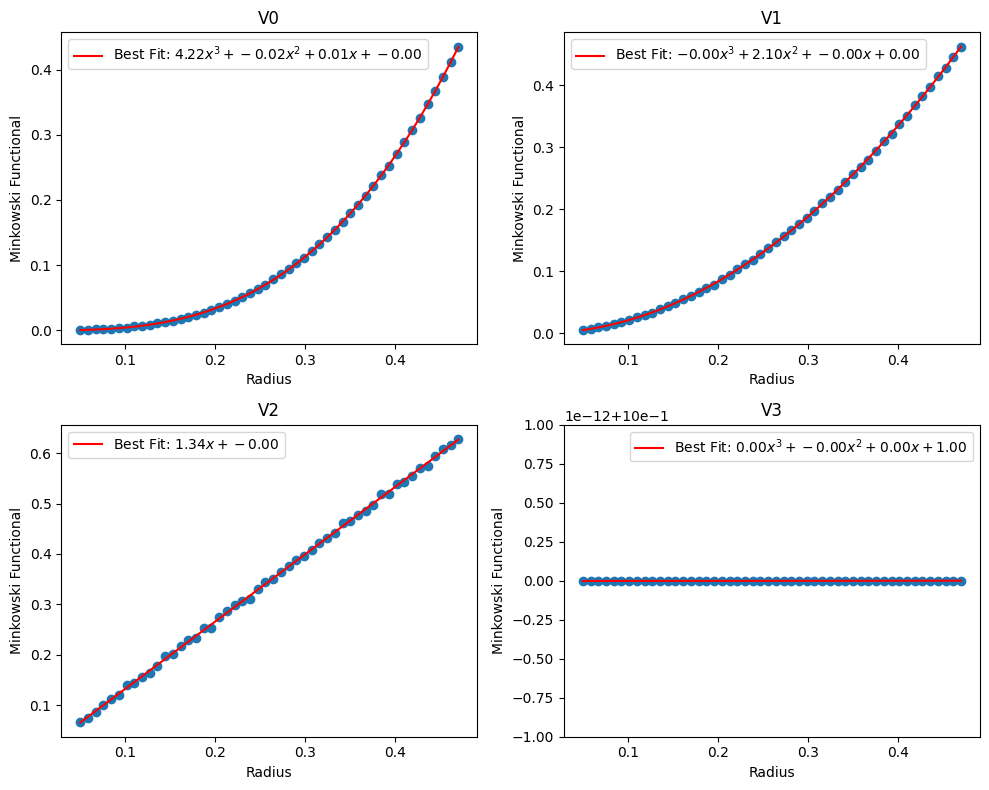
\includegraphics[width=0.6\textwidth]{Images/single_sphere_radius_variance.png}
    \caption{The four Minkowski functionals are plotted against the radius, along with their respective best-fit lines.}
    \label{fig:single_sphere_plot}
\end{figure}


\subsection{A Lattice of Embedded Spheres}
In this case, 125 spheres were embedded in the volume, arranged in the form of a lattice (5 spheres in each direction) within a grid of resolution 500 points per dimension. The total grid length was set to 1 meter, resulting in the spheres being evenly spaced across the grid.

We expect similar trends as with a single sphere: the volume of each sphere should scale with the cube of its radius, the surface area should scale with the square of the radius, and the mean curvature should increase linearly with the radius. For the Euler characteristic, the expected behavior is that it remains constant for each individual sphere, however at at a value of 125, to indicate there's 125 separate objects in the volume.

Spheres of various radii, ranging from 0.05 m to 0.47 m, were embedded in this lattice, and their combined Minkowski functionals were calculated. The functionals for this arrangement of spheres were then plotted against the corresponding radii. Additionally, the best-fit polynomial curves for each functional were plotted, illustrating the overall behavior of the lattice structure, as shown in Figure \ref{fig:lattice_spheres_plot}. We see that $V_0$ follows a cubic polynomial with negligible lower-order terms, while $V_1$ adheres to a quadratic fit. $V_2$ is well described by a linear fit, and $V_3$, as expected, remains constant. The trends observed are consistent with expectations for a lattice of spheres

\begin{figure}[h!] 
    \centering 
    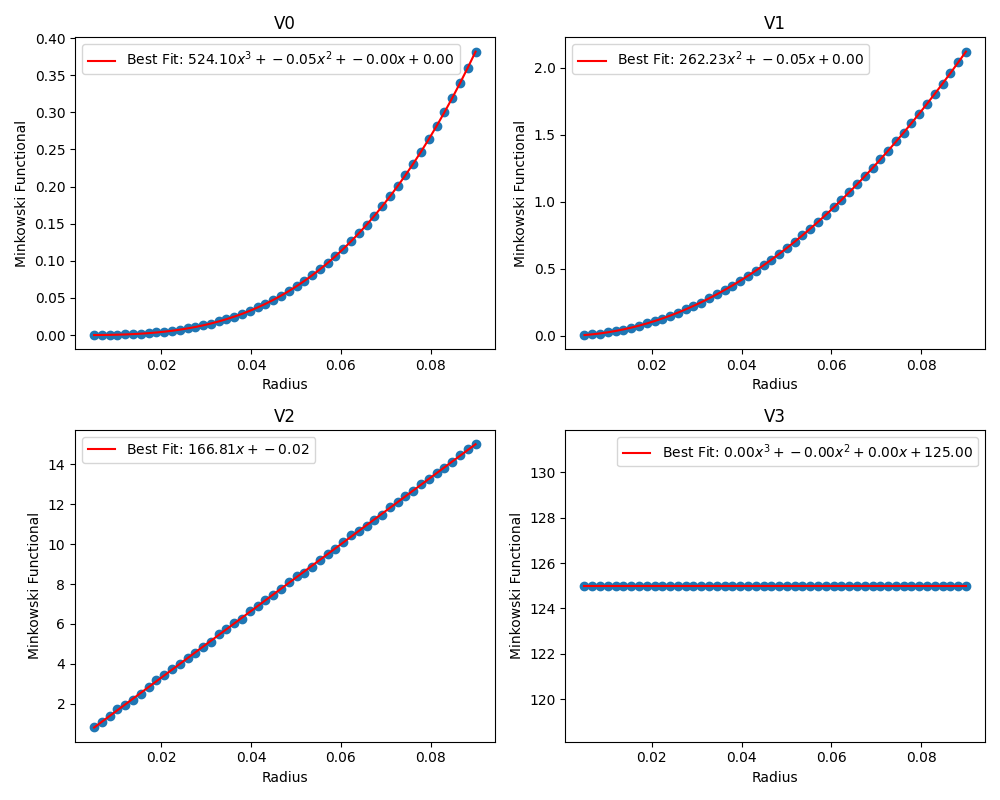
\includegraphics[width=0.6\textwidth]{Images/grid_radius_variance.png} 
    \caption{The four Minkowski functionals for a lattice of spheres are plotted against the radius, along with their respective best-fit lines.} 
    \label{fig:lattice_spheres_plot} 
\end{figure}

\section{Summary}

As part of the semester project so far, A tool has been developed to calculate the Minkowski Functionals and Shapefinders for any general structure, using python, and it's validity has been verified with a standard test case of spehres. This code can be now used to characterize the isodensity contours in the simulation data, which would be the next step in the project. 


\bibliographystyle{plain}  % Style of the bibliography (plain, unsrt, alpha, etc.)
\bibliography{references}  % Path to your .bib file

\end{document}
